Este doble proceso puede decodificar el mensaje original en los mismo s\'{i}mbolos, pero con un radio de compresi\'{o}n promedio de $\frac{7}{8}$.

Como un segundo ejemplo considere una fuente que produce una secuencia de A's y B's con probabilidad p para A y q por B. Si p << q tenemos que

\begin{equation}
\begin{array}{rcl}
H = - \log p^p (1 - p)^{1-p}
= -p \log p(1-p)^{(1-p)/p}
= p \log \frac{e}{p}
\end{array}
\end{equation}

En tal caso uno puede construir una codificaci\'{o}n del mensaje sobre
un canal de 0, 1 lo suficientemente buena mediante el env\'{i}o de una
secuencia especial, por ejemplo 0000, para el s\'{i}mbolo poco
frecuente A y a continuaci\'{o}n, una secuencia indicando el
n\'{u}mero siguiente de B's. Esto podr\'{i}a ser indicado por una
representaci\'{o}n binaria con todos los n\'{u}meros que contienen la
secuencia especial eliminada. Todos los n\'{u}meros hasta el 16 son
representados como de costumbre; el 16 es representado por el
siguiente n\'{u}mero binario despues de 16 que no contiene 4 ceros, es
decir, 17 = 10001, etc.

Se puede demostrar que a medida que $p\rightarrow{0}$ los enfoques de
codificaci\'{o}n ideales proporcionan la longitud de la secuencia
especial es ajustada correctamente.

\part{El canal discreto con ruido}
\label{part:2}

\chapter{Representaci\'{o}n de un canal discreto con ruido}
\label{sec:11}

Ahora consideremos el caso en donde la se\~{n}al es perturbada por
ruido durante la transmisi\'{o} o en algunas de las terminales. Esto
significa que la se\~{n}al recibida no es necesariamente el mismo que
el enviado por el transmisor. Dos casos pueden ser distinguidos. Si
una se\~{n}al particular transmitida siempre produce la misma
se\~{n}al recibida, es decir, la se\~{n}ar recibida es una funcion
definida de la se\~{n}al transmitida, entonces el efecto puede ser
llamado distorsi\'{o}n. Si la funci\'{o}n tiene inversa -las dos
se\~{n}ales transmitidas no deben de producir la misma se\~{n}al
recibida- la distorsi\'{o} puede ser corregida, al menos al principio,
solamente por la realizaci\'{o}n de la operaci\'{o}n de la funci\'{o}n
inversa de la se\~{n}al recibida.

El caso de inter\'{e}s aqu\'{i} es aquel en el que la se\~{n}al no
siempre se someta al mismo cambio en la transmisi\'{o}n. En este caso
podemos asumir que la se\~{n}al recibida $E$ es una funci\'{o} de la
se\~{n}al de transmisi\'{o}n $S$ y una segunda variable, el ruido $N$:
\begin{equation}
E = f(S, N).
\end{equation}

El ruido es considerado como una variable de probabilidad igual al
mensaje que estaba por encima. En general, esto puede ser representado
como un proceso estoc\'{a}stico adecuado. El tipo m\'{a}s general de
canales discretos con ruido que consideramos es una generalizaci\'{o}n
de el canal libre de ruido de estado finito descrito
anteriormente. Podemos asumir un n\'{u}mero finito de estados y un
conjunto de probabilidades

\begin{equation}
P_{\alpha, i}(\beta , j).
\end{equation}

Esta es la probabilidad, si el canal est\'{a} en el estado $\alpha$ y
el s\'{i}mbolo $i$ es transmitido, el s\'{i}mbolo $j$ sera recibido y
el canal se queda en estado $\beta$. As\'{i} $\alpha$ y el rango de
$\beta$ sobre las posibles se\~{n}ales recibidas. En el caso de que
los s\'{i}mbolos sucesivos son perturbados de forma independiente por
el ruido solo hay un estado, y el canal es descrito por el conjunto de
probablidades de transici\'{o}n $P_{i}(j)$, la
probabilidad de transmitir un s\'{i}mbolo $i$ sera recibido como $j$·

Si el canal con ruido es alimentado por una fuente hay dos procesos en
trabajo: la fuente y el ruido. Por lo tanto hay un n\'{u}mero de
entrop\'{i}as que se pueden calcular. En primer lugar est\'{a} la
entrop\'{i}a $H(x)$ de la fuente o de la entrada al canal (\'{e}stos
ser\'{a}n iguales si el transmisor es no singular). La entrop\'{i}a de
la salidad del canal, es decir, la se\~{n}al recibida se denota por
$H(y)$. En el caso sin ruido $H(y) = H(x)$. El conjunto de
entrop\'{i}as de entrada y salida ser\'{a} $H(x, y)$. Finalmente donde
haya dos entrop\'{i}as condicionales $H_{x}(y)$ y $H_{y}(x)$, la
entrop\'{i}a de la salida cuando la entrada es conocida y a la
inversa. Entre esas cantidades tenemos las relaciones
\begin{equation}
H(x, y) = H(x) + H_{x}(y) = H(y) + H_{y}(x).
\end{equation}

Todas estas entrop\'{i}as se pueden medir en funci\'{o}n de por
segundo o en funci\'{o}n de cada s\'{i}mbolo.

\clearpage

\chapter{Equivocaci\'{o}n y capacidad de canal}
\label{sec:12}

Si el canal es con ruido por lo general no es posible el reconstruir
el mensaje original o la se\~{n}al transmitida con certeza por
cualquier operaci\'{o} efectuada sobre la se\~{n}al recibida $E$. Hay,
sin embargo, maneras de transmitir la informaci\'{o}n que
son \'{o}ptimas en el combate contra el ruido. Este es el problema que
consideramos ahora

Supongamos que hay dos posibles s\'{i}mbolos 0 y 1, y estamos
transmitiendo a una velocidad de 1000 s\'{i}mbolos por segundo con
probabilidad de $p_{0} = p_{1} = \frac{1}{2}$. Por lo tanto nuestra
fuenta est\'{a} produciendo informaci\'{o}n a la velocidad de 1000
bits por segundo. Durante la transmisi\'{o}n del ruido se introduce
errores de manera que, en promedio, 1 en 100 se recibieron
incorrectamente (un 0 como 1, o 1 como 0). {\textquestiondown}Cu\'{a}l
es la tasa de transmisi\'{o}n de informaci\'{o}n? Ciertamenet menos de
1000 bits por segundo aproximadamente el 1\% de los s\'{i}mbolos
recibidos son correctos. Nuesto primer impulso podr\'{i}a decir que la
tasa es de 990 bits por segundo, simplemente el n\'{u}mero de errores
esperados. Esto no es satisfactorio ya que no se tiene en cuenta la
falta de conocimiento de d\'{o}nde se producen los errores del
destinatario. Es posible llevarlo a un caso extremo y supongamos que
el ruido es tan grande que los s\'{i}mbolos recibidos son totalmente
independientes de los s\'{i}mbolos transmitidos. La probalidad de
recibir $1$ es $\frac{1}{2}$ en todo lo que se transmite y de manera
similar para 0. Luego, alrededor de la mitada de los s\'{i}mbolos
recibidos son correctos debido al azar, y nos estar\'{i} dando el
cr\'{e}dito del sistema para la transmisi\'{o}n de 500 bits por
segundo, cuando en realidad la informaci\'{o} no se transmite en
absoluto. Igualmente la transmisi\'{o}n "correcta" se obtendr\'{i}a
mediante la dispensaci\'{o}n con el canal entero y lanzando una moneda
en el punto de recepci\'{o}n.

Es evidente que la correci\'{o}n adecuada para aplicar a la cantidad
de informaci\'{o} transmitida es la cantidad de la informaci\'{o}n que
falta de la se\~{n}al recibida, o bien la incertidumbre cuando hemos
recibido una se\~{n}al de lo que fue enviado realmente. De nuestra
discusi\'{o}n anterior de la entrop\'{i}a condicional del mensaje, a
sabiendas de la se\~{n}al recibida, como una medida de esta
informaci\'{o}n faltante. Esta es de la definici\'{o}n apropiada, como
veremos m\'{a}s adelante. Siguiendo esta idea la tasa de
transmisi\'{o}n real, R, se obtiene restando de la tasa de
producci\'{o}n (es decir, la entrop\'{i}a de la fuente) de la tasa
media de la entrop\'{i}a condicional:
\begin{equation}
R = H(x)- H_y(x).
\end{equation}
La entrop\'{i}a condicional $H_y(x)$ ser\'{a}, por conveniencia,
llamada la equivocaci\'{o}n. Que mide la ambig\"{u}edad media de la
se\~{n}al recibida.

En el ejemplo considerado anteriormente, si se recibe un 0 la
probabilidad a posteriori de que un 0 se transmite es 0.99, y que un 1
fue transmitido es 0.01. Estas cifras se invierten si se recibe un
1. Por lo tanto
\begin{equation}
\begin{array}{rcl}
H_y(x) = [.99 log .99+ 0.01 log 0.01]
= .081 bits/s\'{\i}mbolo,
\end{array}
\end{equation}
o 81 bits por segundo. Podemos decir que el sistema est\'{a} transmitiendo a una velocidad de $1000-81 = 919$ bits por segundo. En el caso extremo donde un 0 es igualmente probable que se reciba como un 0 o 1 y de manera similar para 1, las probabilidades a posteriori son $\frac{1}{2}$, $\frac{1}{2}$ y
\begin{equation}
\begin{array}{rcl}
H_y(x) = - \left [\frac{1}{2} log \frac{1}{2} + \frac{1}{2} log \frac{1}{2} \right]
= 1 \mbox{bits por segundo}
\end{array}
\end{equation}
o 1000 bits por segundo. La velocidad de transmisi\'{o}n es entonces como deber\'{i}a ser 0.

El siguiente teorema da una interpretaci\'{o}n directa de la
equivocaci\'{o}n y adem\'{a}s sirve para justificarlo como
la \'{u}nica medida adecuada. Consideramos un sistema de
comunicaci\'{o}n y un observador (o dispositivo auxiliar) que ver
tanto lo que se env\'{i}a y lo que se recupera (con errores debido al
ruido). Este observador toma nota de los errores en el mensaje
recuperado y transmitir los datos al punto de recepci\'{o}n sobre un
"canal de correci\'{o}" para permitir al receptor el corregir los
errores. La se indica esquem\'{a}ticamente en la figura \ref{fig:8}.

\begin{theorem}
\label{th:10}
Si el canal de correci\'{o}n tiene una capacidad igual a $H_y(x)$ es
posible el codificar los datos de correcci\'{o}n para enviarlo a
trav\'{e}s de este canal y corregir todos menos una arbitrariamente
peque\~{n}a fracci\'{o} de los errores. Esto no es posible si la
capacidad del canal es menor que $H_y(x)$.
\end{theorem}

\begin{figure}[!ht]
\centerline{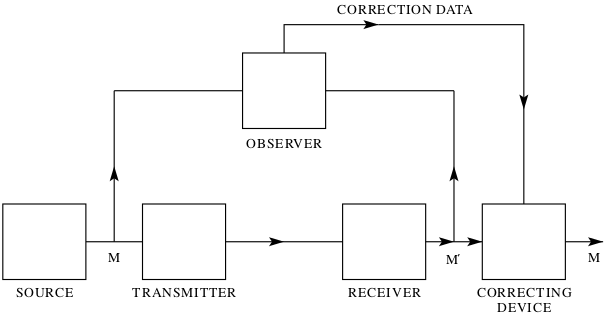
\includegraphics[width=120mm]{Imagenes/SinComentarios/Pagina21-Figura8.png}}
\caption{Un diagrama esquem\'{a}tico de un sistema de correcci\'{o}n.}
\label{fig:8}
\end{figure}

Entonces aproximadamente, $H_y(x)$ es la cantidad de informaci\'{o}n
adicional que debe ser suministrada por segundo al punto de
recepci\'{o}n para corregir el mensaje recibido.

Para probar la primera parte, considere largas secuencias de mensaje
recibido ${M}'$ y el mensaje original correspondiente $M$. Habr\'{a}
lograr\'{i}tmicamente $TH_y(x)$ de ${M}'s$ del cual razonablemente
podr\'{i}a haber producido cada ${M}'$. As\'{i} tenemos que $TH_y(x)$
son los d\'{i}gitos binarios para enviar cada $T$ segundos. Esto se
puede hacer con $\epsilon$ frecuencia de errores en un canal de
capacidad $H_y(x)$.

La segunda parte se puede probar se\~{n}alando en primer lugar para
cada variable discreta $x, y, z$ oportunidad
\begin{equation}
H_y( x,  z) \geq H_y(x).
\end{equation}
La parte izquierda se puede ampliar para dar
\begin{equation}
\begin{array}{rcl}
H_y(z) + H_{yz}(x) \geq H_y(x),
H_{yz}(x) \geq H_y(x) - H_y(z) \geq H_y(x) - H(z).
\end{array}
\end{equation}

Si identificamos $x$ como la salida de la fuente, $y$ como la
se\~{n}al recibida y $z$ como la se\~{n}al enviada por el canal de
correci\'{o}n, entonces la parte derecha es la equivocaci\'{o}n menos
la tasa de transmisi\'{o}n sobre el canal de correci\'{o}n. Si la
capacidad de este canal es menor que la equivocaci\'{o}n de la parte
derecha ser\'{a} mayor que cero y $H_{yz}(x) > 0$. Pero esta es la
incertidumbre de lo que fue enviado, conociendo tanto la se\~{n}al
recibida y la se\~{n}al de correci\'{o}n. Si este es mayor que cero la
frecuencia de errores no puede ser arbitrariamente peque\~{n}o.

\begin{exmp}
Supongamos que los errores suceden al azar en una secuencia de
d\'{i}gitos binarios: la probabilidad $p$ de que un d\'{i}gito es
incorrecto y $q = 1 - p$ es correcto. Estos errores se pueden corregir
si se conoce su posici\'{o}n. As\'{i} el canal de correcci\'{o}n
s\'{o}lo necesita enviar informaci\'{o}n sobre estas posiciones. Esto
equivale a transmitir desde una fuente que produce d\'{i}gitos
binarios con probabilidad $p$ para $1$ (incorrecto) y $q$ para $0$
(correcto). Esto requiere un canal de capacidad
\begin{equation}
- \left [ p \; log\; p \;+ q\;log\;q \right]
\end{equation}
que es la equivocaci\'{o}n del sistema original.

La tasa de transmisi\'{o}n R se puede escribir en otras dos formas
debido a las identidades indicadas anteriormente. Tenemos
\begin{equation}
\begin{array}{rcl}
R = H(x) - H_y(x)
= H(y) - H_x(y)
= H(x) + H(y) - H(x, y).
\end{array}
\end{equation}
\end{exmp}

La primera expresi\'{o}n que define ya ha sido interpretada como la
cantidad de informaci\'{o}n enviada menos la incertidumbre de lo que
fue enviado. La segunda mide la cantidad recibida menos la parte de
este que es debido al ruido. El tercero es la suma de las dos
cantidades menos la entrop\'{i}a conjunta y por lo tanto en un sentido
es el n\'{u}mero de bits por segundo comunes en ambos. As\'{i}, las
tres expresiones tienen un cierto significado intuitivo.

La capacidad $C$ de un canal con ruido debe ser la m\'{a}xima tasa
posible de transmisi\'{o}n, es decir, la tasa cuando la fuente
corresponde adecuadamente al canal. Por lo tanto, definimos la
capacidad del canal por
\begin{equation}
C = \max (H(x) - H_y(x)),
\end{equation}
donde el m\'{a}ximo es con respecto a todas las posibles fuentes de
informaci\'{o}n utilizadas como entrada para el canal. Si el canal no
produce ruido, $H_y(x) = 0$. La definici\'{o}n es entonces equivalente
a la proporcionada para un canal sin ruido desde la entrop\'{i}a
m\'{a}xima para el canal de su capacidad.

\clearpage

\chapter{El teorema fundamental para un canal discreto con ruido}
\label{sec:13}

Puede parecer sorprendente que debemos definir una capacidad definida
C para un canal ruidoso ya que nunca podemos enviar cierta
informaci\'{o}n en un caso as\'{\i}. Est\'{a} claro, sin embargo, que
mediante el env\'{\i}o de la informaci\'{o}n en una forma redundante
la probabilidad de errores se puede reducir. Por ejemplo, mediante la
repetici\'{o}n del mensaje muchas veces y por un estudio
estad\'{i}stico de las diferentes versiones recibidas del mensaje la
probabilidad de errores podr\'{i}a hacerse muy peque\~{n}a. Se
podr\'{i}a esperar, sin embargo, que para hacer esta probabilidad de
errores de enfoque de cero, la redundancia de la codificaci\'{o}n debe
aumentar indefinidamente, y la tasa de transmisi\'{o}n por lo tanto,
tiende a cero. Esto no es en absoluto cierto. Si lo fuera, no
habr\'{i}a una capacidad muy bien definida, pero s\'{o}lo una
capacidad para una frecuencia dada de errores, o una equivocaci\'{o}n
dada; la capacidad de bajar como los requisitos de error se hacen
m\'{a}s estrictas. En realidad, la capacidad $C$ definido
anteriormente tiene un significado muy definido. Es posible enviar
informaci\'{o}n a la velocidad $C$ a trav\'{e}s del canal con tan
peque\~{n}a frecuencia de errores o equivocaci\'{o}n como se desee
mediante la codificaci\'{o}n adecuada. Esta declaraci\'{o}n no es
v\'{a}lida para cualquier tasa mayor que $C$. Si se hace un intento de
transmitir a una velocidad mayor que $C$, por ejemplo $C + R_1$,
entonces no necesariamente ser\'{a} una equivocaci\'{o}n igual o mayor
que al exceso de $R_1$. La naturaleza toma por pago mucha
incertidumbre al exigir justamente eso, por lo que no estamos
consiguiendo m\'{a}s correctamente a trav\'{e}s de $C$.

La situaci\'{o}n se indica en la figua \ref{fig:9}. La tasa de
informaci\'{o}n en el canal se representa horizontalmente y la
equivocaci\'{o}n verticalmente. Cualquier punto por encima de la
l\'{i}nea gruesa de la regi\'{o}n sombreada se puede alcanzar y
aquellos por debajo no. Los puntos de la l\'{i}nea no pueden en
general ser alcanzados, pero por lo general ser\'{a} de dos puntos en
la l\'{i}nea que pueda.

Estos resultados son la principal justificaci\'{o}n para la
definici\'{o}n de C y ahora se han demostrado.

\begin{theorem}
\label{th:11}
Que un canal discreto tenga la capacidad $C$ y una fuente discreta de
la entrop\'{i}a por segundo $H$. Si $H \leq C$ existe un sistema de
codificaci\'{o}n de tal manera que de la salidad de la fuente puede
ser transmitido a trav\'{e}s del canal con una peque\~{n}a frecuencia
de errores arbitraria (o una peque\~{n}a equivocaci\'{o}n
arbitraria). Si $H > C$ es posible codificar la fuente de modo que la
equivocaci\'{o}n es menor que $H - C$ donde $\epsilon$ is
arbitrariamente peque\~{n}o. No existe un m\'{e}todo de
codificaci\'{o}n que da una equivocaci\'{o}n menor de $H - C$.
\end{theorem}

FALTA

\begin{figure}[!ht]
\centerline{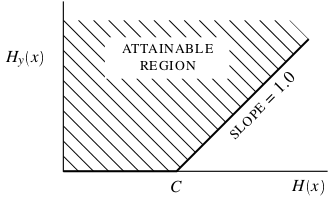
\includegraphics[width=100mm]{Imagenes/SinComentarios/Pagina22-Figura9.png}}
\caption{La equivocaci\'{o}n posible para una entropia de entrada dada
  a un canal.}
\label{fig:9}
\end{figure}

FALTA

\begin{figure}[!ht]
\centerline{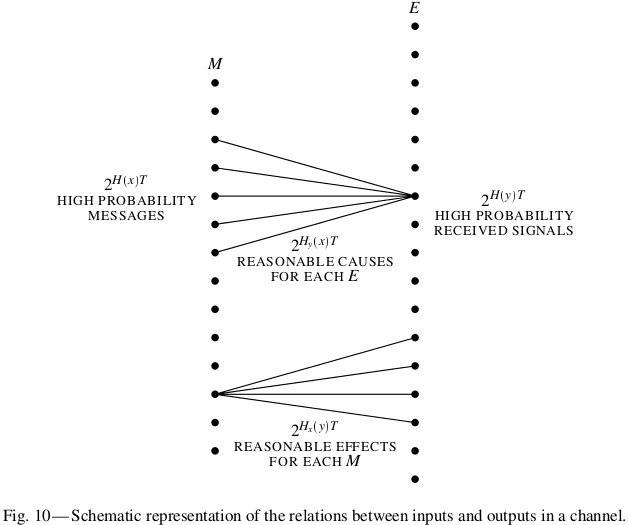
\includegraphics[width=140mm]{Imagenes/Pagina23-Figura10.png}}
\caption{Una representaci\'{o}n esquem\'{a}tica de las relaciones
  entre las entradas y salidas en un canal.}
\label{fig:10}
\end{figure}

FALTA

\clearpage

\chapter{Discussion}
\label{sec:14}

La demostraci\'{o}n del teorema \ref{th:11}, si bien no es una prueba
de la existencia pura, tiene algunas de las deficiencias de tales
pruebas. Un intento de obtener una buena aproximaci\'{o}n a la
codificaci\'{o}n ideal siguiendo el m\'{e}todo de la prueba es
generalmente poco pr\'{a}ctico. De hecho, aparte de algunos casos
m\'{a}s bien triviales y ciertas limitantes, no se ha encontrado
descripci\'{o}n expl\'{i}cita de una serie de aproximaci\'{o}n al
ideal. Probablemente, esto no es casualidad, pero est\'{a} relacionado
con la dificultad de dar una construcci\'{o}n expl\'{i}cita para una
buena approximaci\'{o}n a una secuencia aleatoria.

Una aproximaci\'{o}n a lo ideal ser\'{i}a tener la propiedad de si la
se\~{n}al se altera de manera razonable por el ruido, el original
todav\'{i}a puede ser recuperado. En otras palabras el cambio no
ser\'{a} en general acercarlo m\'{a}s a otra se\~{n}al razonable que
el original. Esto se logra al costo de una cierta cantidad de
redundancia en la codificaci\'{o}n. La redundancia se debe introducir
en la forma correcta para combatir el ruido estructural particular
involucrado. Sin embargo, ninguna redundancia en la fuente por lo
general ayuda si es utilizada en el punto de recepci\'{o}n. En
particular, si la fuente ya tiene cierta redundancia y no se hace
ning\'{u}n intento de eliminar el canal en juego, esta redundancia
ayudar\'{a} a combate del ruido. Por ejemplo, en un canal de
tel\'{e}grafo sin ruido se podr\'{i}a ahorrar alrededor del 50\% en el
tiempo por la codificaci\'{o}n apropiada de los mensajes. Esto no se
hace y la mayor parte de la redundancia de Ingl\'{e}s permanece en el
canal de s\'{i}mbolos. Esto tiene la ventaja, sin embargo, de permitir
un considerable ruido en el canal. Una fracci\'{o}n considerable de
las letras puede ser recibido incorrectamente y todav\'{i} ser
recontruido por el contexto. De hecho, esto no es probablemente una
mala aproximaci\'{o}n al ideal en muchos casos, ya que la estructura
estad\'{i}stica de Ingl\'{e}s es bastante involucrado y las secuencias
razonables de ingl\'{e}s no son demasiado lejos (en el sentido
requerido para el teorema) a partir de una selecci\'{o}n aleatoria.

